\documentclass[10pt,x11names,table]{beamer}

\usetheme[progressbar=frametitle]{metropolis}
\usepackage{appendixnumberbeamer}
\usepackage{xcolor}

\usepackage{polyglossia}
\setmainlanguage{spanish}

\usepackage{listings}

\usepackage{booktabs}
\usepackage[scale=2]{ccicons}

\usepackage{pgfplots}
\usepgfplotslibrary{dateplot}

%ANIMACIONES
\usepackage{animate}
\usepackage{graphicx}
\usepackage[caption=false]{subfig}

\usepackage{xspace}

\newcommand*{\eg}{e.g.\@\xspace}
\newcommand*{\ie}{i.e.\@\xspace}

\let\oldquote\quote
\let\endoldquote\endquote
\renewenvironment{quote}[2][]
  {\if\relax\detokenize{#1}\relax
     \def\quoteauthor{#2}%
   \else
     \def\quoteauthor{#2~---~#1}%
   \fi
   \oldquote}
  {\par\nobreak\smallskip\hfill(\quoteauthor)%
   \endoldquote\addvspace{\bigskipamount}}
   
\usepackage{wrapfig}

\usepackage{subfig}
\usepackage{hyperref}
\usepackage{multicol}

\setbeamertemplate{bibliography item}[text]

\usepackage[font=small,skip=0pt, labelformat=empty]{caption}

\usepackage{dirtytalk}
\usepackage[acronym]{glossaries}
\makeglossaries

\newacronym{acgan}{ACGAN}{Auxiliary Classifier GAN}
\newacronym{ae}{AE}{Autoencoder}
\newacronym{ai}{AI}{Artificial Intelligence}
\newacronym{api}{API}{Application Programming Interface}
\newacronym{bert}{BERT}{Bidirectional Encoder Representations from Transformers}
\newacronym{brief}{BRIEF}{Binary Robust Independent Elementary Features}
\newacronym{brnn}{BRNN}{Bidirectional RNN}
\newacronym{bptt}{BPTT}{Backpropagation Through Time}
\newacronym{cbow}{CBOW}{Continous bag-of-words}
\newacronym{cnn}{CNN}{Convolutional Neural Network}
\newacronym{crnn}{CRNN}{Convolutional Recurrent Neural Network}
\newacronym{ddpm}{DDPM}{Denoising Diffusion Probabilistic Model}
\newacronym{ddim}{DDIM}{Denoising Diffusion Implicit Model}
\newacronym{diffit}{DiffiT}{Diffusion Vision Transformer}
\newacronym{dl}{DL}{Deep Learning}
\newacronym{dnn}{DNN}{Deep Neural Network}
\newacronym{dos}{DoS}{Denial of Service}
\newacronym{drnn}{DRNN}{Deep Recurrent Neural Network}
\newacronym{ecg}{ECG}{Electrocardiogram}
\newacronym{elmo}{ELMo}{Embedding from Language Model}
\newacronym{fast}{FAST}{Features from Accelerated Segment Test}
\newacronym{fid}{FID}{Fréchet Inception Distance}
\newacronym{foss}{FOSS}{Free and open-source software}
\newacronym{gan}{GAN}{Generative Adversarial Network}
\newacronym{glove}{GloVe}{Global Vectors for Word Representation}
\newacronym{gpu}{GPU}{Graphics Processing Unit}
\newacronym{gru}{GRU}{Gated Recurrent Unit}
\newacronym{ilsvrc}{ILSVRC}{ImageNet Large Scale Visual Recognition Challenge}
\newacronym{is}{IS}{Inception Score}
\newacronym{kid}{KID}{Kernel Inception Distance}
\newacronym{ldm}{LDM}{Latent Diffusion Model}
\newacronym{lstm}{LSTM}{Long Short-Term Memory}
\newacronym{mape}{MAPE}{Mean Absolute Perentage Error}
\newacronym{ml}{ML}{Machine Learning}
\newacronym{mlp}{MLP}{Multilayer Perceptron}
\newacronym{mmd}{MMD}{Maximum Mean Discrepancy}
\newacronym{mse}{MSE}{Mean Squared Error}
\newacronym{ner}{NER}{Named Entity Recognition}
\newacronym{nlg}{NLG}{Natural Language Generation}
\newacronym{nlp}{NLP}{Natural Language Processing}
\newacronym{nlu}{NLU}{Natural Language Understanding}
\newacronym{nn}{NN}{Neural Network}
\newacronym{ocr}{OCR}{Optical Character Recognition}
\newacronym{onnx}{ONNX}{Open Neural Network Exchange}
\newacronym{pmml}{PMML}{Predictive Model Markup Language}
\newacronym{relu}{ReLU}{Rectified Linear Unit}
\newacronym{rest}{REST}{Representational State Transfer}
\newacronym{rnn}{RNN}{Recurrent Neural Network}
\newacronym{sae}{SAE}{Stacked Autoencoder}
\newacronym{sift}{SIFT}{Scale-Invariant Feature Transform}
\newacronym{slam}{SLAM}{Simultaneous Localization and Mapping}
\newacronym{sru}{SRU}{Single Recurrent Unit}
\newacronym{surf}{SURF}{Speeded-Up Robust Features}
\newacronym{svm}{SVM}{Support Vector Machine}
\newacronym{vae}{VAE}{Variational Autoencoder}
\newacronym{vgg}{VGG}{Visual Geometry Group}
\newacronym{vit}{ViT}{Vision Transformer}
\newacronym{wsgi}{WSGI}{Web Server Gateway Interface}
\newacronym{xai}{XAI}{eXplainable Artificial Intelligence}
\newacronym{yolo}{YOLO}{You Only Look Once}
\newacronym{zsl}{ZSL}{Zero-shot Learning}
\subtitle{Métodos Generativos, curso 2024-2025}

\date{\today}
\author{Guillermo Iglesias, guillermo.iglesias@upm.es \newline
Jorge Dueñas Lerín, jorge.duenas.lerin@upm.es  \newline
Félix Fuentes Hurtado, felix.fuentes@upm.es}

\institute{Escuela Técnica Superior de Ingeniería de Sistemas Informáticos | UPM \newline
\hbox{} \newline \ccbysa \hspace{0.1pt} \ccNonCommercial}

%%%%%%%%%%%%%%%%%%%%%%%%%%%%%%%%%%%%%       
\title{Transformers}

\begin{document}
\maketitle

\begin{frame}{Contenidos}
  \begin{enumerate}
      \item Introducción
      \item Auto-encoders (AEs)
      \item{Auto-encoders Variacionales (VAEs)}
      \item{Generative Adversarial Networks (GANs)}
      \item{Transformers}
      \item{Diffusion Models}
    \end{enumerate}
\end{frame}


\begin{frame}{Contenidos}
  \begin{enumerate}
      \item Introducción
      \item Auto-encoders (AEs)
      \item{Auto-encoders Variacionales (VAEs)}
      \item{Generative Adversarial Networks (GANs)}
      \item{\textbf{Transformers}}
      \item{Diffusion Models}
    \end{enumerate}
\end{frame}

\section{Transformers}
% \begin{frame}{Auto-encoders (AEs)}
% \end{frame}


\begin{frame}{Motivación}

Hasta la aparición de los transformers, los problemas secuenciales se trataban (casi) siempre con \textbf{redes recurrentes}.

Sin embargo, dichas arquitecturas tienen dos problemas bien conocidos:

\begin{itemize}
    \item Su entrenamiento no se puede paralelizar, ya que un instante depende del anterior, y así sucesivamente, por lo que su entrenamiento es \textbf{lento}.
    \item Aunque aparecieron para ``recordar'', su memoria es bastante limitada, empeorando sus resultados cuanto más larga es la secuencia con la que tienen que trabajar.
\end{itemize}
\end{frame}

\begin{frame}{¿Qué son los Transformers?}

\begin{itemize}
  \item Los \textbf{transformers} son un tipo de arquitectura de redes neuronales revolucionaria en el campo de la inteligencia artificial.
  \item A mediados de 2017 aparece un artículo científico que demuestra que existe una alternativa a las redes recurrentes para trabajar con \textbf{problemas secuenciales}.
  \item En concreto, habla del concepto de ``\textbf{atención}'', que básicamente significa ``\textbf{ponderar}'' los elementos de las secuencias según afecten más o menos a las predicciones.
  \item Habla sobre todo de NLP (Natural Language Processing), pero también es aplicable a series temporales (y a imágenes con ligeras modificaciones).
  \item Elimina el concepto de \textbf{recursión}, con lo que el entrenamiento puede ser mucho más \textbf{rápido}.
  \item Además, es capaz de ``\textbf{memorizar}'' secuencias más largas.


\end{itemize}
\end{frame}

\begin{frame}{¿Qué son los Transformers?}

\begin{figure}
    \centering
    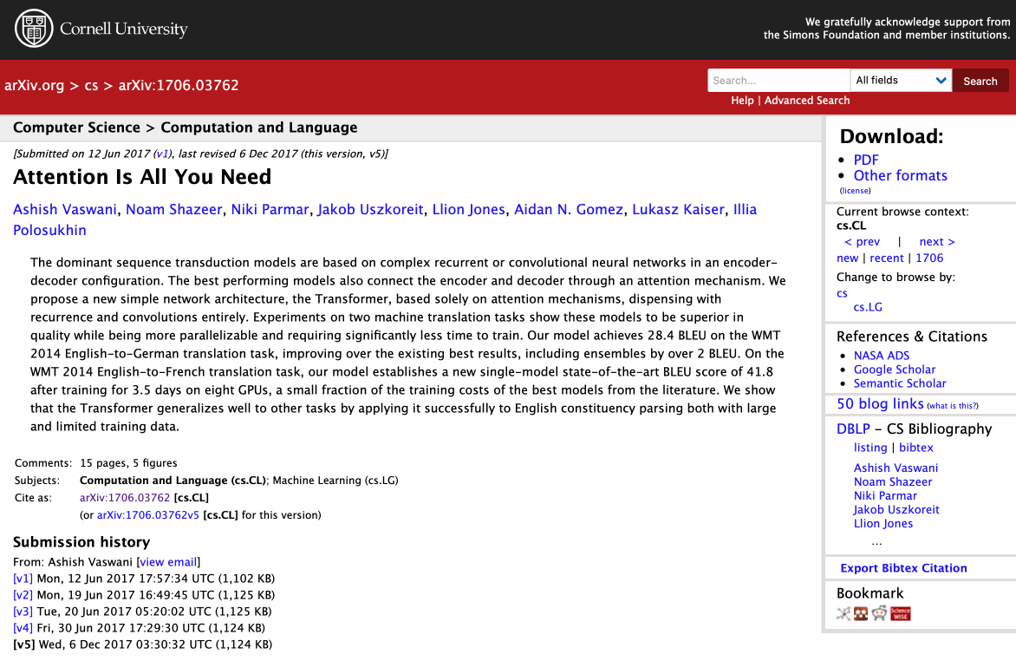
\includegraphics[width=0.7\textwidth]{Slides/figures/02_Metodos_Generativos/transf-attention-is-all-you-need.png}
    \caption{Captura de arxiv.org del artículo ``Attention is all you need''.}
\end{figure}

\end{frame}

\begin{frame}{¿Qué son los Transformers?}

\begin{figure}
    \centering
    
\includegraphics[width=1\textwidth]{Slides/figures/02_Metodos_Generativos/transf-attention-is-all-you-need-citas.png}
    \caption{Captura de Google Scholar mostrando el número de citas a fecha Octubre de 2023.}
\end{figure}

\end{frame}


\begin{frame}{Arquitectura de los Transformers}

\begin{columns}
\column{0.6\textwidth}
\begin{itemize}
    \item Una arquitectura encoder-decoder con atención.
    \item La atención ``mira'' a la secuencia de entrada y decide para cada instante qué otras partes de la misma son importantes (podéis entenderlo como el ``contexto'').
    \item Consiste en bloques encoder y decoder apilables (\texttt{Nx} bloques)
    \item Capas densas y bloques Multi-Head Attention (MHA).
    \item Positional embbeding (para introducir la información ``temporal'' en el caso de las series temporales o ``situacional'' en el caso de NLP)
\end{itemize}

\column{0.4\textwidth}
\vspace{0.2em}
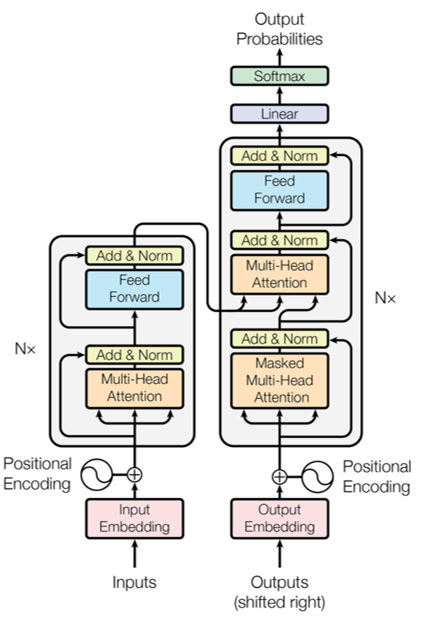
\includegraphics[width=\textwidth]{Slides/figures/02_Metodos_Generativos/trans-arch.png}

\end{columns}
\end{frame}

\begin{frame}{Arquitectura de los Transformers}
\begin{itemize}
    \item El bloque \textbf{Multi-Head Attention} es el que permite al modelo ``fijarse'' en las cosas más importantes.
    \item Funciona creando varios \textbf{mapas de activación} (Q: query, K: key, V: value) y comprobando sus \textbf{relaciones}.
\end{itemize}

\begin{figure}
    \centering
    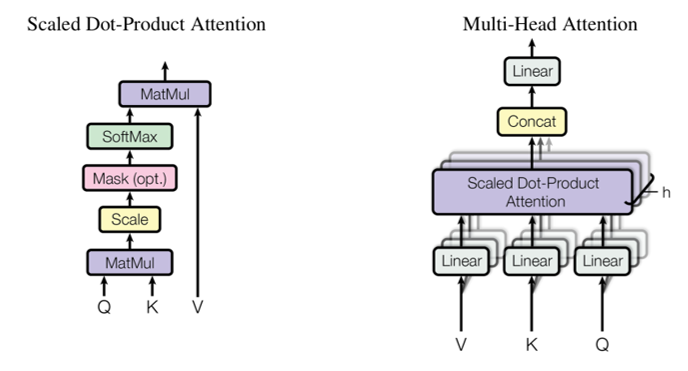
\includegraphics[width=0.6\textwidth]{Slides/figures/02_Metodos_Generativos/trans-arch2.png}
    \caption{Principales mecanismos de la arquitectura transformer.}
\end{figure}

\end{frame}



\begin{frame}{Arquitectura de los Transformers}
\begin{itemize}
    \item Vamos a ver la arquitectura transformer explicada en el campo del procesamiento del lenguaje natural, ya que es el caso de uso más típico.
    \item Para el caso de series temporales o imágenes es muy similar, lo único que cambia es la codificación de los datos de entrada.
\end{itemize}

\begin{figure}
    \centering
    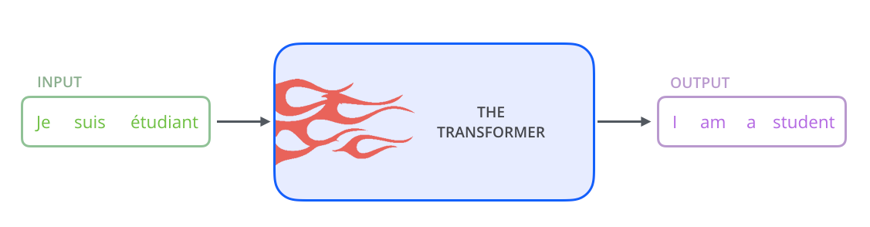
\includegraphics[width=0.9\textwidth]{Slides/figures/02_Metodos_Generativos/trans-arch3.png}
    \caption{Ejemplo simplificado de una tarea de traducción con un transformer (\href{http://jalammar.github.io/illustrated-transformer/}{fuente}).}
\end{figure}
\end{frame}

\begin{frame}{Arquitectura de los Transformers}
\begin{itemize}
    \item Los transformers se componen de un \textbf{encoder} y un \textbf{decoder}.
\end{itemize}

\begin{figure}
    \centering
    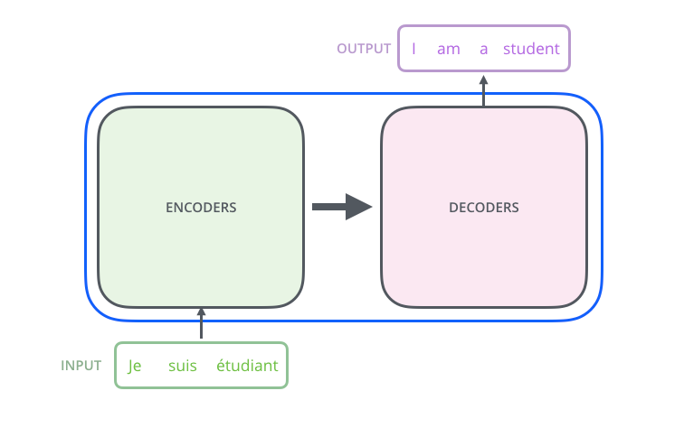
\includegraphics[width=0.7\textwidth]{Slides/figures/02_Metodos_Generativos/trans-arch4.png}
    \caption{Arquitectura encoder-decoder (\href{http://jalammar.github.io/illustrated-transformer/}{fuente}).}
\end{figure}
\end{frame}

\begin{frame}{Arquitectura de los Transformers}
\begin{itemize}
    \item O para ser más exactos, de $N$ bloques de encoders apilados seguidos de $N$ bloques de decoders apilados.
\end{itemize}

\begin{figure}
    \centering
    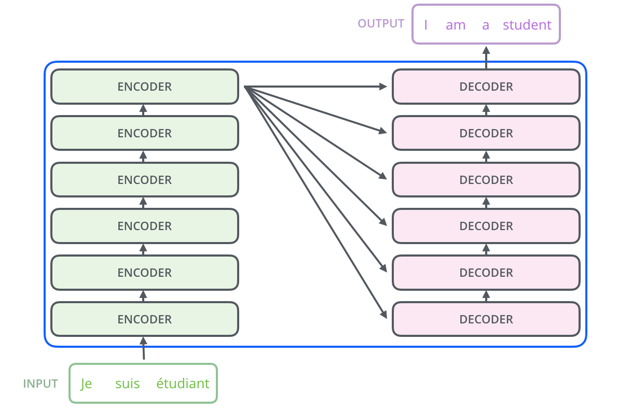
\includegraphics[width=0.6\textwidth]{Slides/figures/02_Metodos_Generativos/trans-arch5.png}
    \caption{Arquitectura general del transformer (\href{http://jalammar.github.io/illustrated-transformer/}{fuente}).}
\end{figure}
\end{frame}

\begin{frame}{Arquitectura de los Transformers}
\begin{itemize}
    \item Dentro de cada \textbf{encoder} tendremos un bloque de capas \textbf{feed-forward} (densas) y otro bloque de \textbf{Self-Attention}, el cual ayuda al encoder a fijarse no solo en la palabra que está procesando en ese momento, sino también en las demás palabras de la secuencia de entrada.
    \item En los \textbf{decoders}, tendremos además de eso, un \textbf{bloque de Encoder-Decoder attention} que le permita decirle qué partes de la secuencia de entrada son \textbf{importantes}.
\end{itemize}

\begin{figure}
    \centering
    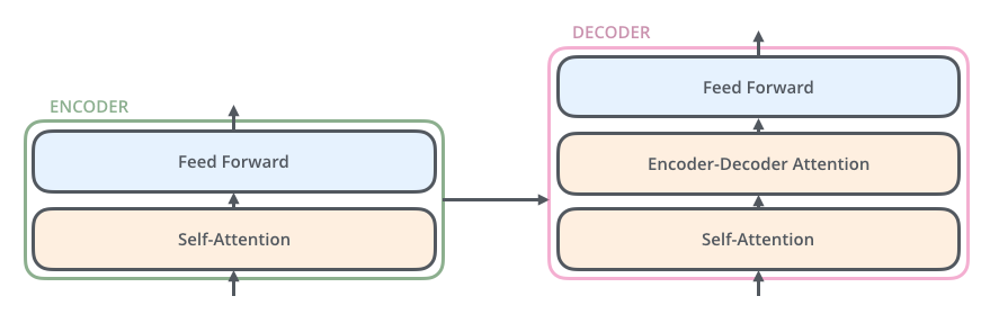
\includegraphics[width=0.75\textwidth]{Slides/figures/02_Metodos_Generativos/trans-arch6.png}
    \caption{Arquitectura general del encoder y el decoder (\href{http://jalammar.github.io/illustrated-transformer/}{fuente}).}
\end{figure}
\end{frame}


\begin{frame}{Arquitectura de los Transformers}
\begin{itemize}
    \item Los vectores de  entrada \textit{fluyen} a través de los bloques cada uno en una posición fija. \item El encoder crea dependencias entre estos ``caminos'' en los bloques de \textbf{self-attention}.
    \item ¡Esto se puede \textbf{paralelizar}, ya no existen dependencias temporales!
\end{itemize}

\begin{figure}
    \centering
    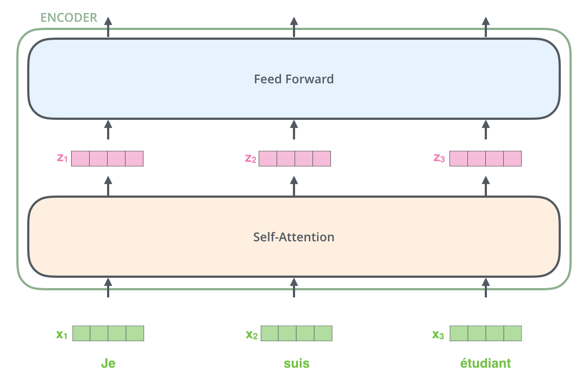
\includegraphics[width=0.5\textwidth]{Slides/figures/02_Metodos_Generativos/trans-arch7.png}
    \caption{Arquitectura de los bloques de tipo \textbf{encoder} en detalle (\href{http://jalammar.github.io/illustrated-transformer/}{fuente}).}
\end{figure}
\end{frame}

\begin{frame}{Arquitectura de los Transformers}
\begin{itemize}
    \item Este proceso se repite para cada bloque “encoder”.
\end{itemize}

\begin{figure}
    \centering
    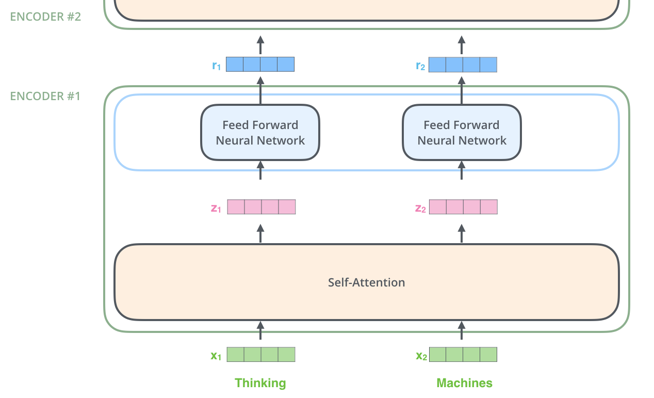
\includegraphics[width=0.7\textwidth]{Slides/figures/02_Metodos_Generativos/trans-arch8.png}
    \caption{Arquitectura del \textbf{encoder} en detalle (\href{http://jalammar.github.io/illustrated-transformer/}{fuente}).}
\end{figure}
\end{frame}

\begin{frame}{¿Cómo funciona la atención?}

\begin{columns}
\column{0.6\textwidth}
\begin{itemize}
    \item En la frase “The \textbf{animal} didn’t cross the street because it was too tired”, el modelo no sabe a priori que “it” se refiere a “The animal” -> ¡Esto es lo que hace el bloque de \textbf{self-attention}!
    \item Conforme el modelo procesa \textbf{cada palabra} (o cada posición en la secuencia de entrada), el módulo de self-attention le permite \textbf{mirar} al \textbf{resto de las posiciones} en la secuencia de entrada para pistas que le permitan \textbf{codificar mejor} el elemento \textbf{actual}.
\end{itemize}

\column{0.4\textwidth}
% \vspace{0.2em}
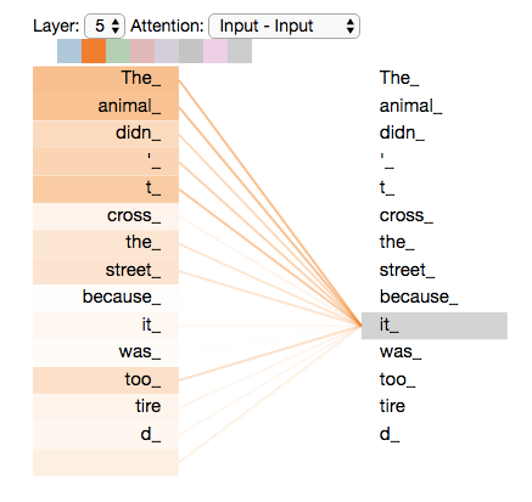
\includegraphics[width=\textwidth]{Slides/figures/02_Metodos_Generativos/trans-att.png}

\end{columns}
\end{frame}



\begin{frame}{¿Cómo funciona el bloque de self-attention?}

\begin{columns}
\column{0.4\textwidth}
\begin{enumerate}
    \item Creamos 3 matrices entrenables ($W^Q$, $W^K$, $W^V$)
    \item Multiplicamos cada vector de entrada por cada una de las 3 matrices entrenables ($W^Q$, $W^K$, $W^V$) 
    \item Obtenemos 3 nuevos vectores ($q_n$, $k_n$, $v_n$), que además son de menor dimensionalidad que los de entrada, ya que las matrices se eligen así para reducir el coste computacional

\end{enumerate}

\column{0.6\textwidth}
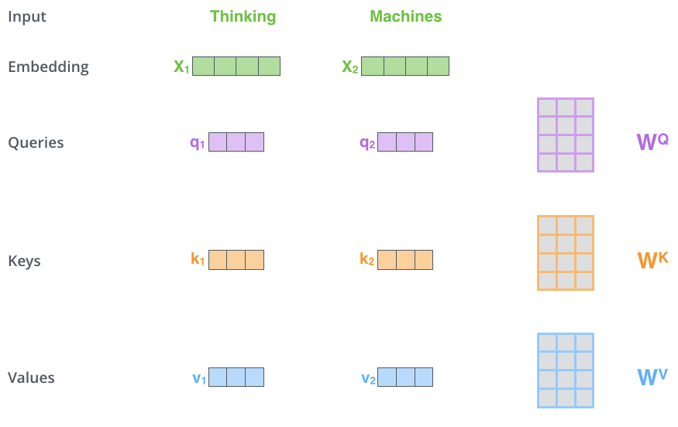
\includegraphics[width=\textwidth]{Slides/figures/02_Metodos_Generativos/trans-att2.png}

\end{columns}
\end{frame}


\begin{frame}{¿Cómo funciona el bloque de self-attention?}

\begin{enumerate}
\setcounter{enumi}{3}
    \item Calculamos la self-attention como el producto escalar de $q_n\cdot k_n$. 
\end{enumerate}

\begin{figure}
    \centering
    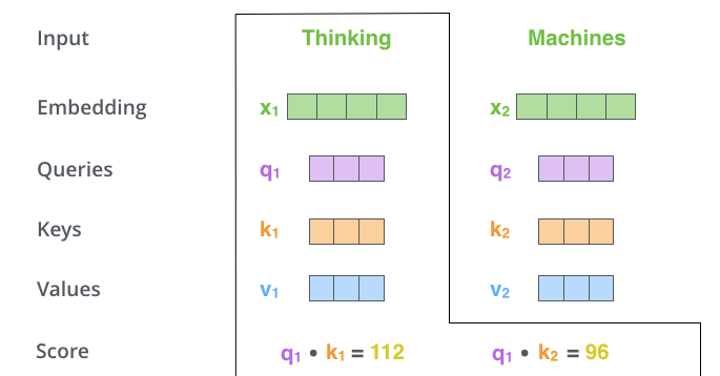
\includegraphics[width=0.85\textwidth]{Slides/figures/02_Metodos_Generativos/trans-att3.png}
    \caption{Ejemplo del producto escalar en el mecanismo de self-attention (\href{http://jalammar.github.io/illustrated-transformer/}{fuente}).}
\end{figure}

\end{frame}


\begin{frame}{¿Cómo funciona el bloque de self-attention?}

\begin{columns}
\column{0.4\textwidth}
\begin{enumerate}
\setcounter{enumi}{4}
    \item Dividimos entre la raiz cuadrada del número de dimensiones escogidas para los vectores \textbf{key} (para estabilizar los gradientes durante el entrenamiento)
    \item Aplicamos la funcion \textbf{softmax} para normalizar los valores y que sumen 1.
\end{enumerate}
\vspace{1em}
¡Ya tenemos el valor de la atención!

Pero no hemos acabado...

\column{0.6\textwidth}
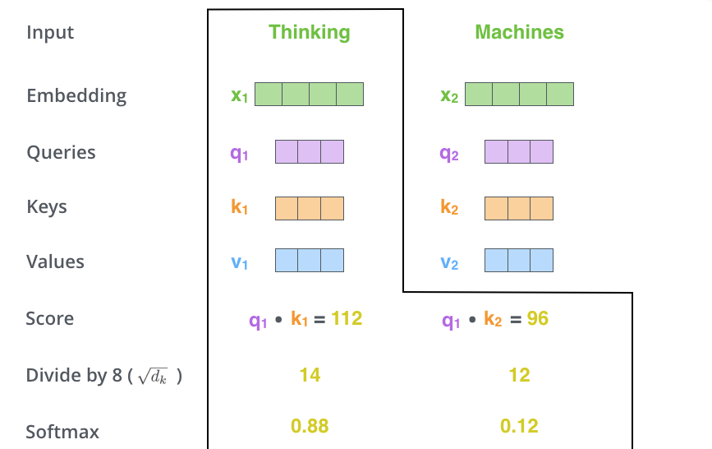
\includegraphics[width=\textwidth]{Slides/figures/02_Metodos_Generativos/trans-att4.png}

\end{columns}
\end{frame}

\begin{frame}{¿Cómo funciona el bloque de self-attention?}

\begin{columns}
\column{0.4\textwidth}
\begin{enumerate}
\setcounter{enumi}{6}
    \item Multiplicamos el valor de la atención de cada vector de entrada ($a_n$) por el vector value $v_1$ (porque estamos calculando el valor de la atención para el \textbf{vector de entrada 1})
    \item Sumamos todos los resultados $a_n \cdot v_n$, obteniendo $z_1$

\end{enumerate}
\vspace{1em}
Y ahora sí que hemos acabado :-)

\column{0.6\textwidth}
\vspace{0.2em}
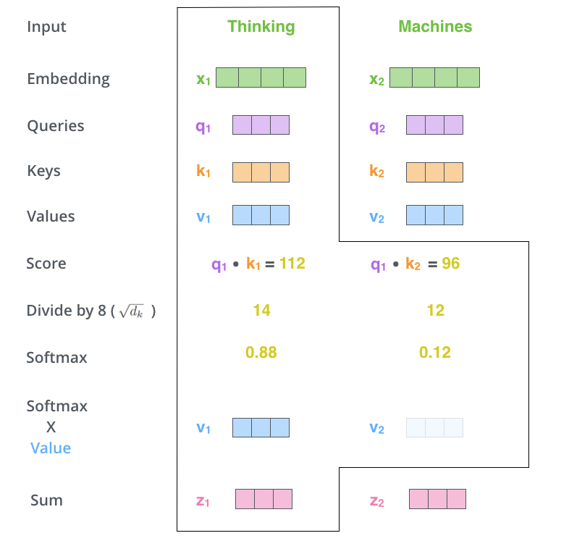
\includegraphics[width=\textwidth]{Slides/figures/02_Metodos_Generativos/trans-att5.png}

\end{columns}
\end{frame}


\begin{frame}{¿Cómo funciona el bloque de self-attention?}

\begin{itemize}
    \item Solamente indicar que esto, en realidad, se hace de forma \textbf{matricial} para ir más rápido.
    \item Y con más de un conjunto de $W^Q$, $W^K$, $W^V$ (\textbf{multi-head}).
\end{itemize}

\begin{figure}
    \centering
    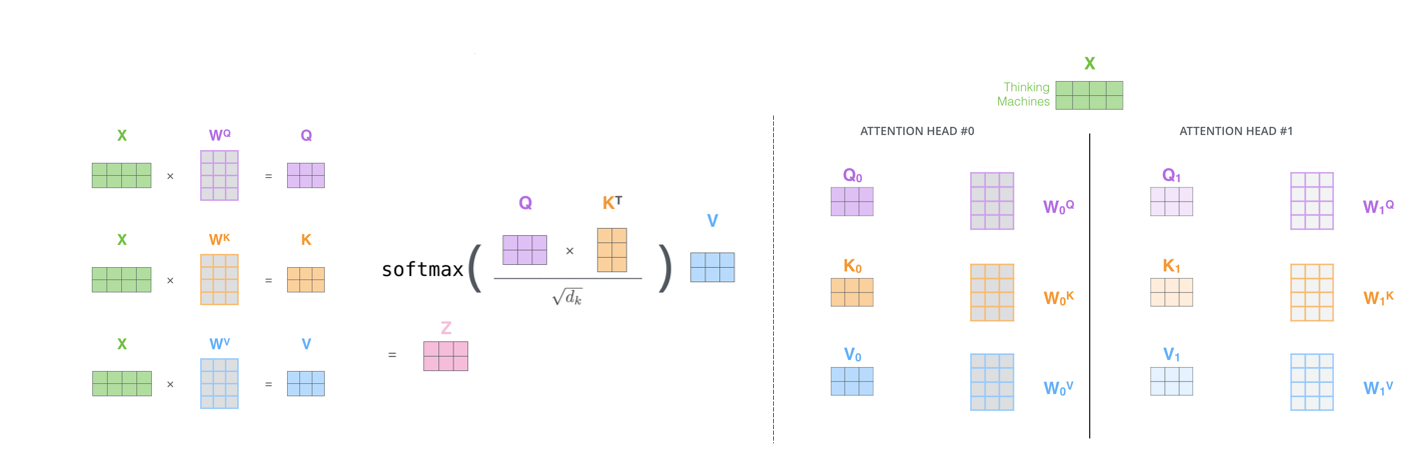
\includegraphics[width=\textwidth]{Slides/figures/02_Metodos_Generativos/trans-att6.png}
    \caption{Ejemplo del cálculo de la \textbf{self-attention} (\href{http://jalammar.github.io/illustrated-transformer/}{fuente}).}
\end{figure}
\end{frame}


\begin{frame}{Resumen}

\begin{figure}
    \centering
    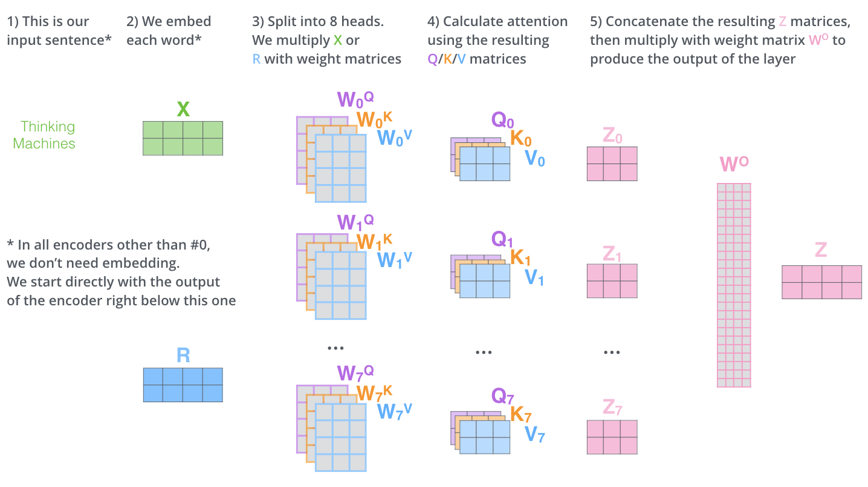
\includegraphics[width=0.9\textwidth]{Slides/figures/02_Metodos_Generativos/trans-att-resumen.png}
    \caption{Resumen del mecanismo de \textbf{self-attention} (\href{http://jalammar.github.io/illustrated-transformer/}{fuente}).}
\end{figure}
\end{frame}


\begin{frame}{Pero... ¿y la información de la posición?}

\begin{itemize}
    \item Si hemos dicho que se procesan todos los inputs de forma paralela, hemos perdido la información del tiempo.
    \item La solución es añadir lo que se conoce como \textbf{positional embedding}, que es lo que le indica a la red la posición de cada elemento de entrada en la secuencia completa.
\end{itemize}
\end{frame}

\begin{frame}{Pero... ¿y la información de la posición?}
\begin{figure}
    \centering
    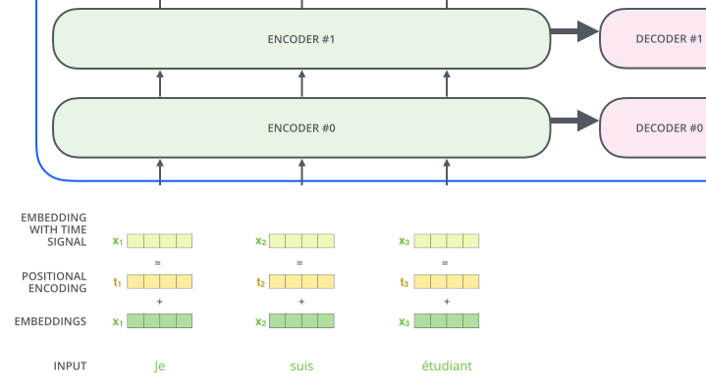
\includegraphics[width=0.9\textwidth]{Slides/figures/02_Metodos_Generativos/trans-encoding.png}
    \caption{Ejemplo de \textbf{positional embedding} (\href{http://jalammar.github.io/illustrated-transformer/}{fuente}).}
\end{figure}
\end{frame}

\begin{frame}{Más información...}

Toda esta explicación está basada en la de ``The illustrated Transformer'', desarrollada por Jay Alammar.

La tenéis disponible en: \href{http://jalammar.github.io/illustrated-transformer/}{http://jalammar.github.io/illustrated-transformer/}.

Si os habéis quedado con dudas, es \textbf{muy recomendable} que os leáis el post y os veáis el video, lo más seguro es que os disipe todas las dudas :-)
\end{frame}



\begin{exercise}
\href{https://colab.research.google.com/drive/1dIKI6xl_Wi5XycbSgYF9qJDYWBsvvTrH}{Ejemplo de transformer}
\end{exercise}

%%%%%%%%%%%%%%%%%%%%%%%%%%%%

\begin{frame}{Recursos}
\begin{itemize}
    \item Diapositivas de Moodle
    \item Google Collaboratory
    \item Deep Learning Book (https://www.deeplearningbook.org/)
    \item https://www.pyimagesearch.com/blog
    \item https://machinelearningmastery.com/blog
\end{itemize}
\end{frame}

% \section{Auto-encoders Variacionales (VAEs)}
% % \begin{frame}{Auto-encoders Variacionales(VAEs)}
% % \end{frame}

% \section{Generative Adversarial Networks (GANs)}
% % \begin{frame}{Generative Adversarial Networks (GANs)}
% % \end{frame}

% \section{Transformers}
% % \begin{frame}{Transformers}
% % \end{frame}

% \section{Diffusion Models}
% % \begin{frame}{Diffusion Models}
% % \end{frame}


\appendix

% \begin{frame}[allowframebreaks]{Referencias}
%     \bibliography{references}
%     \bibliographystyle{abbrv}
% \end{frame}

\begin{frame}<presentation:0>{License}
    \begin{block}{Tema \texttt{slides-upm}. Puedes obtener sus fuentes en}
        \begin{center}\url{http://gitlab.com/blazaid/slides-upm}\end{center}
    \end{block}
  
    Tanto esta presentación como el tema están licenciados bajo \href{http://creativecommons.org/licenses/by-sa/4.0/}{Creative Commons
  Atribución-CompartirIgual 4.0 Internacional (CC BY-SA 4.0)}.
    \begin{center}\ccbysa\end{center}
\end{frame}

\end{document}
